\documentclass[letterpaper,conference]{IEEEtran}
\usepackage{cite}
\usepackage{booktabs}
\usepackage{url}
\usepackage{graphicx}
\usepackage{pgfplots}
\pgfplotsset{compat=1.18}
% Generated by research/scripts/make_paper_assets.py; do not edit.
\newcommand{\NotebookN}{5}
\newcommand{\NotebookProcMean}{5.69}
\newcommand{\NotebookProcSD}{0.04}
\newcommand{\NotebookPromptMean}{1222.12}
\newcommand{\NotebookGenMean}{2425.67}
\newcommand{\NotebookProcMin}{5.61}
\newcommand{\NotebookProcMax}{5.71}
\newcommand{\NotebookPromptSec}{1.222}
\newcommand{\NotebookGenSec}{2.426}
\newcommand{\NotebookRuntimeGenRate}{12.78}
\newcommand{\NotebookDerivedGenRate}{13.19}
\newcommand{\LabradorN}{5}
\newcommand{\LabradorProcMean}{43.86}
\newcommand{\LabradorProcSD}{0.43}
\newcommand{\LabradorPromptMean}{15947.52}
\newcommand{\LabradorGenMean}{19376.81}
\newcommand{\LabradorProcMin}{43.52}
\newcommand{\LabradorProcMax}{44.58}
\newcommand{\LabradorPromptSec}{15.948}
\newcommand{\LabradorGenSec}{19.377}
\newcommand{\LabradorRuntimeGenRate}{1.60}
\newcommand{\LabradorDerivedGenRate}{1.65}
\newcommand{\RPCN}{5}
\newcommand{\RPCProcMean}{168.67}
\newcommand{\RPCProcSD}{0.16}
\newcommand{\RPCPromptMean}{31076.27}
\newcommand{\RPCGenMean}{36913.69}
\newcommand{\RPCProcMin}{168.49}
\newcommand{\RPCProcMax}{168.83}
\newcommand{\RPCPromptSec}{31.076}
\newcommand{\RPCGenSec}{36.914}
\newcommand{\RPCRuntimeGenRate}{0.84}
\newcommand{\RPCDerivedGenRate}{0.87}
\newcommand{\ProcCoordinates}{(Notebook,\NotebookProcMean) (Labrador,\LabradorProcMean) (RPC--2,\RPCProcMean)}
\newcommand{\FailureConnection}{16}
\newcommand{\FailurePreparation}{10}
\newcommand{\FailureLoading}{1}
\newcommand{\FailureIncomplete}{3}
\newcommand{\FailurePartial}{2}


\title{Reproducible RPC Inference Across Resource-Constrained ARM Single-Board Computers}

\author{
\IEEEauthorblockN{Hudson Moreira\IEEEauthorrefmark{1}, Marcelo Knörich Zuffo\IEEEauthorrefmark{2}}
\IEEEauthorblockA{\IEEEauthorrefmark{1}Master's program, Escola Politécnica, University of São Paulo, São Paulo, Brazil\\
\IEEEauthorrefmark{2}Department of Electronic Systems Engineering, Escola Politécnica, University of São Paulo, São Paulo, Brazil}
}

\begin{document}
\maketitle

\begin{abstract}
Splitting a quantized language model across small local computers is attractive when one device has insufficient memory, but networked execution can exchange computation for communication overhead. This paper reports a reproducible, deliberately narrow evaluation of the RPC backend of \texttt{llama.cpp} on homogeneous ARM single-board computers. We compare five valid executions of a notebook-only baseline, five of a single Labrador board, and five of a notebook coordinating two Labrador RPC workers. The selected workload uses Qwen2.5-1.5B-Instruct Q5\_K\_M, a fixed short prompt, deterministic sampling, and a frozen runtime. The logs verify that both RPC workers received assigned layers and executed graph operations for each selected request. Under this configuration, two-worker RPC is slower than the isolated Labrador baseline: 168.67 s versus 43.86 s of process time. The result is a bounded observation, not a claim about all models, networks, or distributed systems. We release the raw evidence, reconstruction scripts, build recipe, and failure inventory for review.
\end{abstract}

\begin{IEEEkeywords}
edge AI, consumer electronics, ARM SBC, local inference, RPC, reproducibility
\end{IEEEkeywords}

\section{Introduction}
Large language model inference is increasingly relevant to local and consumer devices, where privacy, connectivity, and resource ownership can motivate execution near the user. Quantization reduces model storage and memory requirements, while model partitioning can combine several constrained devices. However, a partitioned request must move intermediate state and coordinate remote computation; therefore, adding devices need not reduce latency.

This work studies that trade-off in a controlled laboratory setup. It does not propose a new partitioning algorithm or claim a general scalability limit. Instead, it asks a narrower question: for one quantized instruction model, one short deterministic prompt, and a homogeneous ARM testbed, does coordinating two RPC workers complete the request faster than running the same model on one Labrador board?

The contributions are: (1) an auditable dataset with explicit inclusion and exclusion rules; (2) direct evidence that both selected RPC workers participated in the same inference, rather than merely accepting a connection; and (3) a reproducible comparison separating prompt processing, generation, actual token count, and process time. The answer is negative for the tested configuration: two-worker RPC is slower than the isolated board.

\section{Related Work}
The RPC backend used here is an experimental feature of \texttt{llama.cpp} that exposes remote devices and allows a client to offload computation to one or more servers \cite{ggmlrpc2026}. Qwen2.5 provides the model family context for the selected instruction-tuned checkpoint \cite{qwen25}. Prior edge-inference work addresses broader system designs: EdgeShard formulates device selection and model partitioning for heterogeneous edge resources \cite{edgeshard}, while MDI-LLM studies model-distributed inference and recurrent pipeline parallelism across low-power devices \cite{mdillm}. Those studies motivate collaborative edge inference but do not replace a measurement of this specific RPC implementation, hardware, and workload. Our contribution is consequently an evaluation artifact and bounded baseline rather than a new distributed-inference method.

\section{Testbed and Protocol}
\subsection{Hardware and software}
The testbed contains homogeneous Caninos Labrador 7 boards: ARM64 Cortex-A53, four cores, approximately 1.99 GiB RAM, Debian GNU/Linux 12, and Linux 6.1.76. The inventory records no swap on the boards. They were connected through the \texttt{end0} Ethernet interface; the 100 Mb/s/full-duplex figure comes from dated kernel link-up records in the inventory, not from a throughput benchmark. The article uses pseudonymous roles: the notebook is the client; Labrador-A and Labrador-B are the two RPC workers. The internal raw artifacts retain the original operational identifiers, while this paper avoids publishing IP addresses and hostnames. The notebook executes the client, scheduler, local CPU backend, and any model portion not assigned remotely; it is not a passive controller.

The client log identifies a 12th Gen Intel Core i7-1255U notebook with 31,829 MiB visible memory, Linux x86\_64, one local CPU backend, and a four-thread llama.cpp compute pool. The log does not preserve the notebook distribution release or a separate worker-thread setting. The ARM server invocation and inventory do not provide a worker thread count; therefore, the client value must not be treated as a worker value. The present notebook state is Ubuntu 26.04 with 12 logical CPUs, but this post-hoc state is not asserted as the experimental OS.

The model is Qwen2.5-1.5B-Instruct in Q5\_K\_M GGUF format (SHA-256 \texttt{b4666107...896f8c}). The fixed x86 client binary has SHA-256 \texttt{13b3c2e9...348d69}; its log reports GNU 15.2. The ARM package was cross-compiled from \texttt{llama.cpp} commit \texttt{68e79bd8}, with RPC enabled, native CPU detection disabled, and OpenMP, CUDA, Vulkan, Metal, and RDMA disabled. The local compilation variant applies the preserved \texttt{-O0} patch to the common and RPC HTTP compilation targets. The package uses GCC 12 and a Debian 12 arm64 sysroot; the ABI audit reports maximum GLIBC 2.34 and GLIBCXX 3.4.30. These are materially different x86 and ARM builds, so the comparison is an end-to-end configuration comparison rather than an isolated architecture effect.

\subsection{Frozen workload}
Every selected case used context 512, four threads, \texttt{-ngl 99}, a maximum of 32 output tokens, temperature zero, seed 42, \texttt{--ignore-eos}, and no warmup. The prompt was ``Write exactly one short sentence about distributed computing.'' The runtime reports 38 prompt tokens and, for every included case, 32 actually generated tokens. Each process was newly started; disk caches were not cleared, so the experiment is not a cold-disk benchmark. The process-time metric includes startup, model loading, RPC setup, prompt processing, generation, and residual work not separately instrumented.

\subsection{Validity and selection}
The five notebook cases come from \texttt{matrix-validation-1}; the five isolated ARM cases come from \texttt{matrix-validation-5}; and the five RPC cases combine two valid cases from \texttt{matrix-validation-7} with three valid cases from \texttt{rpc2-complete-1}. These groups share model hash, client hash, runtime source commit, prompt, sampling parameters, and context. They do not form one consecutive campaign: the launcher and health-check procedure changed before the final three RPC cases, so campaign provenance is retained and the groups are not presented as uninterrupted repetitions.

\section{Worker Participation Evidence}
The RPC selection requires more than an open TCP port or a successful client exit. Qwen2.5 has 28 repeating transformer blocks, represented by tensors \texttt{blk.0} through \texttt{blk.27}. The runtime also exposes logical layer 28 for the output stage; in the selected requests, layers 0--14 were assigned to Labrador-A and layers 15--28 to Labrador-B. Thus layer 28 is not a 29th transformer block: it covers the output-stage tensors such as \texttt{output\_norm} and \texttt{output}. The paired server-log slices contain distinct graph-compute, graph-recompute, and tensor-transfer events for both hosts. For a representative selected request, each host recorded 3 graph-compute events, 30 graph-recompute events, and 33 get-tensor events; set-tensor counts were 345 and 356. Event counts establish activity but do not imply identical computational work. Each request records 38 evaluated prompt tokens, 32 predicted tokens, and normal completion with exit code zero. The earlier instrumented pilot independently established the same participation pattern; it is cited as validation evidence and was not repeated for this paper.

The selected cases have 426 relevant operation records in the Labrador-A server slice and 435 in Labrador-B under the reconstruction script's broad graph/tensor event rule. These counts are evidence of execution activity, not a claim that the two servers performed identical work. The notebook remains part of the computation, so the comparison is notebook-only versus one ARM board versus notebook-plus-two-workers, not one board versus an entirely remote cluster.

\section{Results}
\begin{table}[t]
\caption{Selected valid executions and process-time statistics. Values are reconstructed from raw logs; SD is sample standard deviation.}
\label{tab:process}
\centering
\footnotesize
\begin{tabular}{lrrrrr}
\toprule
Condition & $n$ & Mean (s) & SD (s) & Min (s) & Max (s)\\
\midrule
Notebook & \NotebookN & \NotebookProcMean & \NotebookProcSD & \NotebookProcMin & \NotebookProcMax\\
Labrador & \LabradorN & \LabradorProcMean & \LabradorProcSD & \LabradorProcMin & \LabradorProcMax\\
RPC--2 & \RPCN & \RPCProcMean & \RPCProcSD & \RPCProcMin & \RPCProcMax\\
\bottomrule
\end{tabular}
\end{table}

\begin{figure}[t]
\centering
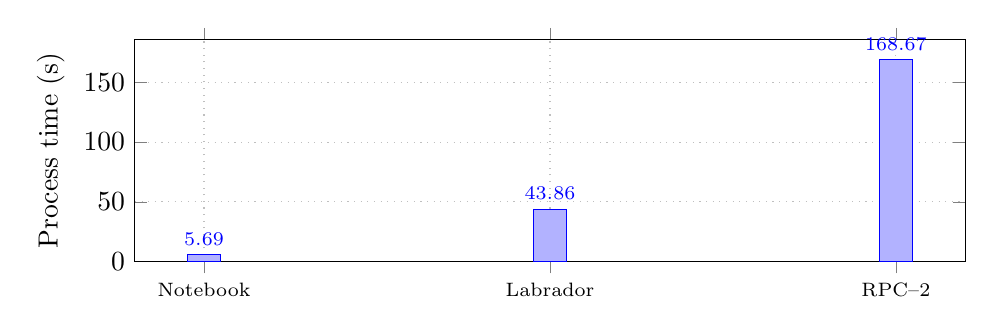
\begin{tikzpicture}
\begin{axis}[ybar,bar width=12pt,width=\columnwidth,height=4.4cm,ylabel={Process time (s)},symbolic x coords={Notebook,Labrador,RPC--2},xtick=data,xticklabel style={font=\scriptsize},ymin=0,grid=major,major grid style={dotted},nodes near coords, nodes near coords style={font=\scriptsize}]
\addplot coordinates \ProcCoordinates;
\end{axis}
\end{tikzpicture}
\caption{Mean process time for the five selected valid cases per condition. Standard deviations are tabulated in Table~\ref{tab:process}; the plot has no error bars and emphasizes scale, not statistical significance.}
\label{fig:process}
\end{figure}

Table~\ref{tab:phases} separates the runtime's prompt and generation measurements. The reported generation-rate column is the arithmetic mean of the individual \texttt{predicted\_per\_second} values extracted from the final JSON response of each valid request. It is not recomputed from the 32-token limit or from an average time. We do not call the remaining process time ``loading time'': loading and first-token timestamps were not independently instrumented.

\begin{table}[t]
\caption{Mean phase metrics in seconds for valid selected cases. Runtime generation rate is the mean of the per-request \texttt{predicted\_per\_second} field.}
\label{tab:phases}
\centering
\footnotesize
\begin{tabular}{lrrrr}
\toprule
Condition & Prompt & Gen. & Tok. & RT gen.\\
\midrule
Notebook & \NotebookPromptSec & \NotebookGenSec & 32 & \NotebookRuntimeGenRate\\
Labrador & \LabradorPromptSec & \LabradorGenSec & 32 & \LabradorRuntimeGenRate\\
RPC--2 & \RPCPromptSec & \RPCGenSec & 32 & \RPCRuntimeGenRate\\
\bottomrule
\end{tabular}
\end{table}

The table reports the mean of the runtime's per-request \texttt{predicted\_per\_second}; it is not 32 divided by the mean generation time. The reconstruction CSV also retains that derived ratio under a separate name, but it is not used as the runtime-reported rate. The fifteen selected cases are valid performance observations, not a reliability sample. The complete inventory contains 55 logged attempts across campaigns and conditions, with failures preserved as follows:

\begin{table}[t]
\caption{Failure inventory reconstructed from all scanned attempts; campaigns are not pooled into a single success denominator.}
\label{tab:failures}
\centering
\footnotesize
\begin{tabular}{lr}
\toprule
Failure class & Count\\
\midrule
Connection/startup & \FailureConnection\\
Preparation/tool/host & \FailurePreparation\\
Loading timeout/kill & \FailureLoading\\
Incomplete timeout/interrupt & \FailureIncomplete\\
Partial generation & \FailurePartial\\
\bottomrule
\end{tabular}
\end{table}

The five valid cases per condition were selected using explicit selection criteria: valid status, complete phase metrics, actual token count, and worker evidence. They were not five consecutive successes. The failure table distinguishes preparation and host availability, connection/startup, loading timeout, incomplete termination, and partial generation; a zero exit code alone was not sufficient for inclusion. Because these attempts span different campaigns and launcher procedures, no single operational success percentage is reported here.

\section{Discussion and Limitations}
The observed result is specific and reproducible: in this configuration, RPC-2 is slower than the isolated Labrador board. The latency difference is consistent with a combination of remote graph execution, intermediate-state communication, serialization, and coordination. The dataset does not isolate those mechanisms; in particular, the study does not justify attributing the result exclusively to the 100 Mb/s link.

The experiment has one model, one short prompt, one quantization, one network segment, and five valid cases per condition. Data were collected in distinct campaigns, and detailed logging was used for RPC validation. Loading, time to first token, peak memory, and a direct communication-only cost are absent. Memory snapshots are before/after observations, not peak measurements. The study does not evaluate user-facing services, quality, energy, privacy leakage, concurrent requests, or model sizes that require more memory. Local services on consumer devices motivate the work, but no particular consumer application was tested.

\section{Conclusion}
We presented a reproducible audit of a small ARM RPC inference setup. The raw logs establish that both RPC workers participated in each of five selected two-worker requests. Under the frozen Qwen2.5-1.5B Q5\_K\_M workload, RPC-2 required 168.67 s of process time on average, compared with 43.86 s for a single Labrador board. This is an observation about the tested configuration, not a universal statement about distributed inference. The released evidence and failure inventory provide a basis for future work on phase-level loading and communication measurements without overstating scalability.

\section*{Acknowledgment and AI-use disclosure}
OpenAI Codex, an AI coding agent, was used to organize logs and manifests, draft and revise portions of the Introduction, Related Work, Testbed and Protocol, Results, Discussion, and Conclusion sections, and prepare or revise the Python analysis and LaTeX asset scripts. All reported values in this manuscript were reconstructed from preserved logs by the repository scripts. The authors remain responsible for verification, technical claims, citations, and the final text. This disclosure identifies the AI system and the affected content in accordance with IEEE guidance on AI-generated text \cite{ieeeai}.

\bibliographystyle{IEEEtran}
\bibliography{references}

\end{document}
